\documentclass[a4paper,twoside,10pt, twocolumn]{report}
% Dino Anastasopoulos, 2021

% Include Packages
%\usepackage[a4paper,inner=3.5cm,outer=2.5cm,top=2.5cm,bottom=2.5cm]{geometry}  % Set page margins
\usepackage{fullpage}
\usepackage{float}                  % Allows 'Here and Only Here' [H] for Floats
\usepackage[hyphens]{url}           % \url{} command
\usepackage{charter}                  % Set font to Times
\usepackage{graphicx}               % \includegraphics
%\usepackage{subfigure}              % Allow subfigures
\usepackage{caption}
\usepackage{subcaption}

\usepackage{amsmath}
\usepackage{amssymb}
\usepackage{amsthm}
\usepackage{booktabs}
\usepackage{parskip}
\usepackage[all]{nowidow}
\setnoclub[2]
\setnowidow[2]

% Referencing
% Provides \Vref and \vref to indicate where a reference is.
\usepackage{varioref} 
% Hyperlinks references
\usepackage[bookmarks=true,bookmarksopen=true]{hyperref} 
% Provides \Cref, \cref, \Vref, \vref to include the type of reference: fig/eqn/tbl
\usepackage{cleveref} 
\usepackage{pgfgantt}

% Setup Hyperref
\hypersetup{
	colorlinks   = true,              %Colours links instead of ugly boxes
	urlcolor     = blue,              %Colour for external hyperlinks
	linkcolor    = blue,              %Colour of internal links
	citecolor    = blue                %Colour of citations
}
% Names for Clever Ref
\crefname{table}{table}{tables}
\Crefname{table}{Table}{Tables}
\crefname{figure}{figure}{figures}
\Crefname{figure}{Figure}{Figures}
\crefname{equation}{equation}{equations}
\Crefname{equation}{Equation}{Equations}

% Wits Citation Style
\usepackage{natbib} % Force natbib.sty to put citation labels in the reference list
\makeatletter
\renewcommand\NAT@biblabel[1]{\def\citeauthoryear##1##2{##1 ##2}[#1]\hfill}
\renewcommand\NAT@bibsetup[1]{%
  \setlength{\itemsep}{\bibsep}\setlength{\parsep}{\z@}}
\def\@lbibitem[#1]#2{%
  \if\relax\@extra@b@citeb\relax\else
    \@ifundefined{br@#2\@extra@b@citeb}{}{%
     \@namedef{br@#2}{\@nameuse{br@#2\@extra@b@citeb}}}\fi
   \@ifundefined{b@#2\@extra@b@citeb}{\def\NAT@num{}}{\NAT@parse{#2}}%
   \item[\hfil\hyper@natanchorstart{#2\@extra@b@citeb}\@biblabel{#1}%
    \hyper@natanchorend]%
    \NAT@ifcmd#1(@)(@)\@nil{#2}}
\makeatother


\bibliographystyle{named-wits}
\bibpunct{[}{]}{;}{a}{}{}  % to get correct punctuation for bibliography
\setlength{\skip\footins}{1.5cm}
\newcommand{\citets}[1]{\citeauthor{#1}'s \citeyearpar{#1}}
\renewcommand\bibname{References}  

\pagestyle{headings}

\pagestyle{plain}
\pagenumbering{roman}

\newenvironment{declaration}{\ \vfill\begin{center}\textbf{Declaration}\end{center}\addcontentsline{toc}{section}{Declaration}}{\vfill\vfill\newpage}

\begin{document}
	\onecolumn
	\thispagestyle{empty}
	
	\setcounter{page}{0}
	\addcontentsline{toc}{chapter}{Preface}
	
	\begin{center}
		\vfill
		{
			\huge \bf \textsc{Cartoonify: \\Artistic Image Filters Using Several Processing Techniques}\\
			\large School of Computer Science \& Applied Mathematics\\
			\large University of the Witwatersrand\\[20pt]
			\normalsize
			Dino Anastasopoulos\\
			\today
		}
		
		\vfill
		\vfill
		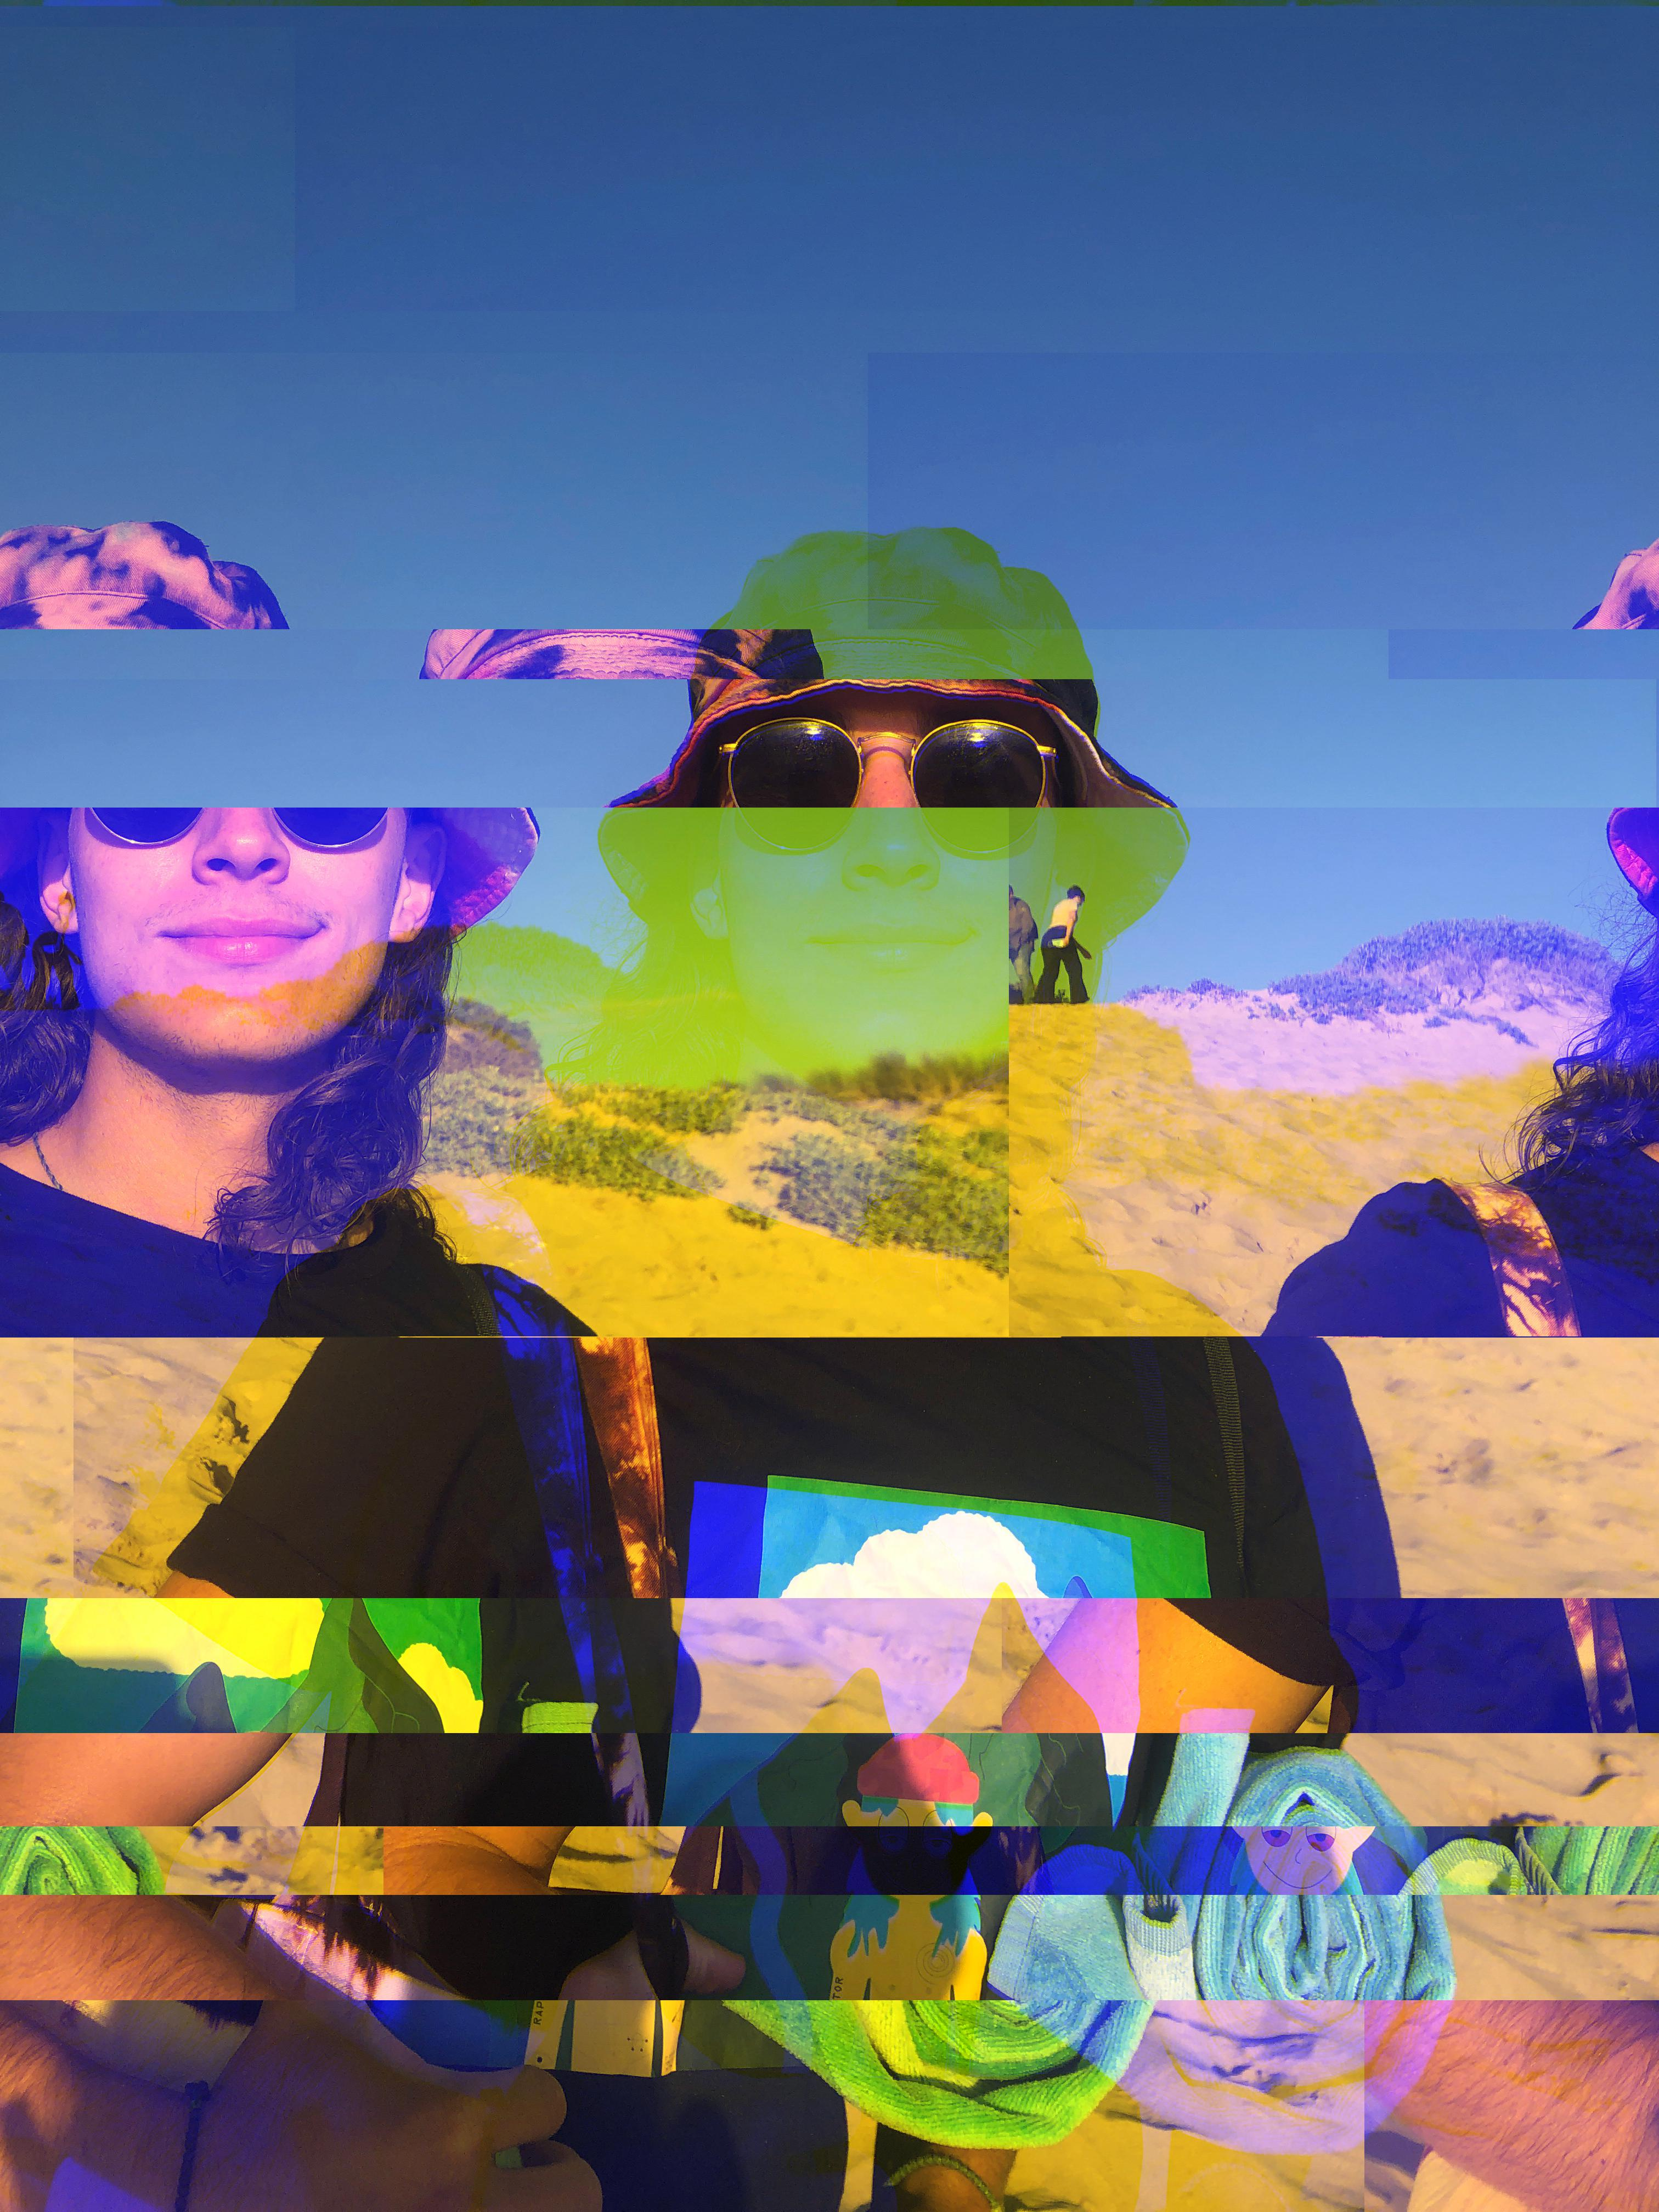
\includegraphics[width=0.5\textwidth]{../Images/Output_Individual/Glitch_Portrait.jpg}

	\end{center}
	

	\newpage

	\pagestyle{plain}
	\setcounter{page}{1}
	\setcounter{tocdepth}{3}
	\setcounter{secnumdepth}{3}
	
	\phantomsection
	\begin{declaration}
		
		\vspace{0.5cm}
		\noindent I, Dino Anastasopoulos, declare that this project is my own, unaided work. It is being submitted for the degree of Honors at the University of the Witwatersrand. It has not been submitted for any degree or examination at any other university.
		
		\par\vspace{2cm}
		\begin{flushright}
			
\includegraphics[width=30mm]{Images/DinoSign.png}\par 
			Dino Anastasopoulos\par\vspace{0.1cm}
			\today
		\end{flushright}
	\end{declaration}
	
	\phantomsection
	\addcontentsline{toc}{section}{Table of Contents}
	\tableofcontents
	\newpage
	\phantomsection
	\addcontentsline{toc}{section}{List of Figures}
	\listoffigures
	\newpage

	\pagenumbering{arabic}

	\twocolumn
	\chapter{Introduction}
	The following report will explain the techniques used to achieve various artistic image filters and effects. The file size of this document is extremely large, since the images have all been saved in their original quality, to allow for the results to be seen clearly after zooming in to individual images.
	
	Each section will simply show the result for the same image, "Portrait", however, the appendix contains a separate page for each effect applied on many different images across several domains.
	
	
	\chapter{Body}
	
	\section{Main Effects}
	This section contains the main effects of the project, which have been implemented from scratch using Digital Image Processing techniques.
	\subsection{Main Effect \#1 - Cartoonify}
	\subsubsection{Techniques}
	Grayscale
	Gaussian blurring to remove fine details from image since cartoons are simple.
	Edge detection on blurred gray image.
	Using k-means clustering to perform colour quantization.
	Gaussian blurring to remove further details.
	Combine extracted edges with clustered and blurred colour image.
	This process can be seen in Figure \ref{Process_Cartoonify}.
	
	\begin{figure}[h]
		\caption{Cartoonify Process}
		\centering
		\includegraphics[width=\linewidth]{../Images/Process/Effect1_Cartoonify.jpg}
		\label{Process_Cartoonify}
	\end{figure}
	
	
	\subsection{Main Effect \#2 - Pencil Sketch}
	
	
	This process can be seen in Figure \ref{Process_Pencil_Sketch}.
	
	\begin{figure}[h]
		\caption{Pencil Sketch Process}
		\centering
		\includegraphics[width=\linewidth]{../Images/Process/Effect2_Pencil_Sketch.jpg}
		\label{Process_Pencil_Sketch}
	\end{figure}
	
	
	
	\subsection{Main Effect \#3 - Pixelate}
	This process can be seen in Figure \ref{Process_Pixelate}.
	
	\begin{figure}[h]
		\caption{Pixelate Process}
		\centering
		\includegraphics[width=\linewidth]{../Images/Process/Effect3_Pixelate.jpg}
		\label{Process_Pixelate}
	\end{figure}
	
	
	
	
	\subsection{Main Effect \#4 - Emboss}

	This process can be seen in Figure \ref{Process_Emboss}.
	
	\begin{figure}[h]
		\caption{Emboss Process}
		\centering
		\includegraphics[width=\linewidth]{../Images/Process/Effect4_Emboss.jpg}
		\label{Process_Emboss}
	\end{figure}
	
	
	
	
	\section{Extra Effects}
	This section contains extra effects which require very little code, use built-in methods which are a part of the OpenCV library, or use external libraries. These have been included out of interest, and because the results are aesthetically pleasing.
	\subsection{Extra Effect \#1 - ColorMaps}
	Using cv2.applyColorMap(img, chosenMap)\\
	These can be seen in Figure \ref{Images_ColourMaps}.
	\subsubsection{Duo Chromatic}
	Random ColorMap selected from [cv2.COLORMAP\_AUTUMN, cv2.COLORMAP\_WINTER, cv2.COLORMAP\_SUMMER, cv2.COLORMAP\_SPRING]\\
	As seen in Figure \ref{Duo}.
	\subsubsection{Thermal 1}
	cv2.COLORMAP\_HSV\\
	As seen in Figure \ref{Thermal1}.
	\subsubsection{Thermal 2}
	cv2.COLORMAP\_RAINBOW\\
	As seen in Figure \ref{Thermal2}.
	\subsubsection{Thermal 3}
	cv2.COLORMAP\_JET\\
	As seen in Figure \ref{Thermal3}.
	\subsubsection{UV}
	cv2.COLORMAP\_COOL\\
	As seen in Figure \ref{UV}.
	
	\begin{figure}[h]	
	\subfloat[Duo]{	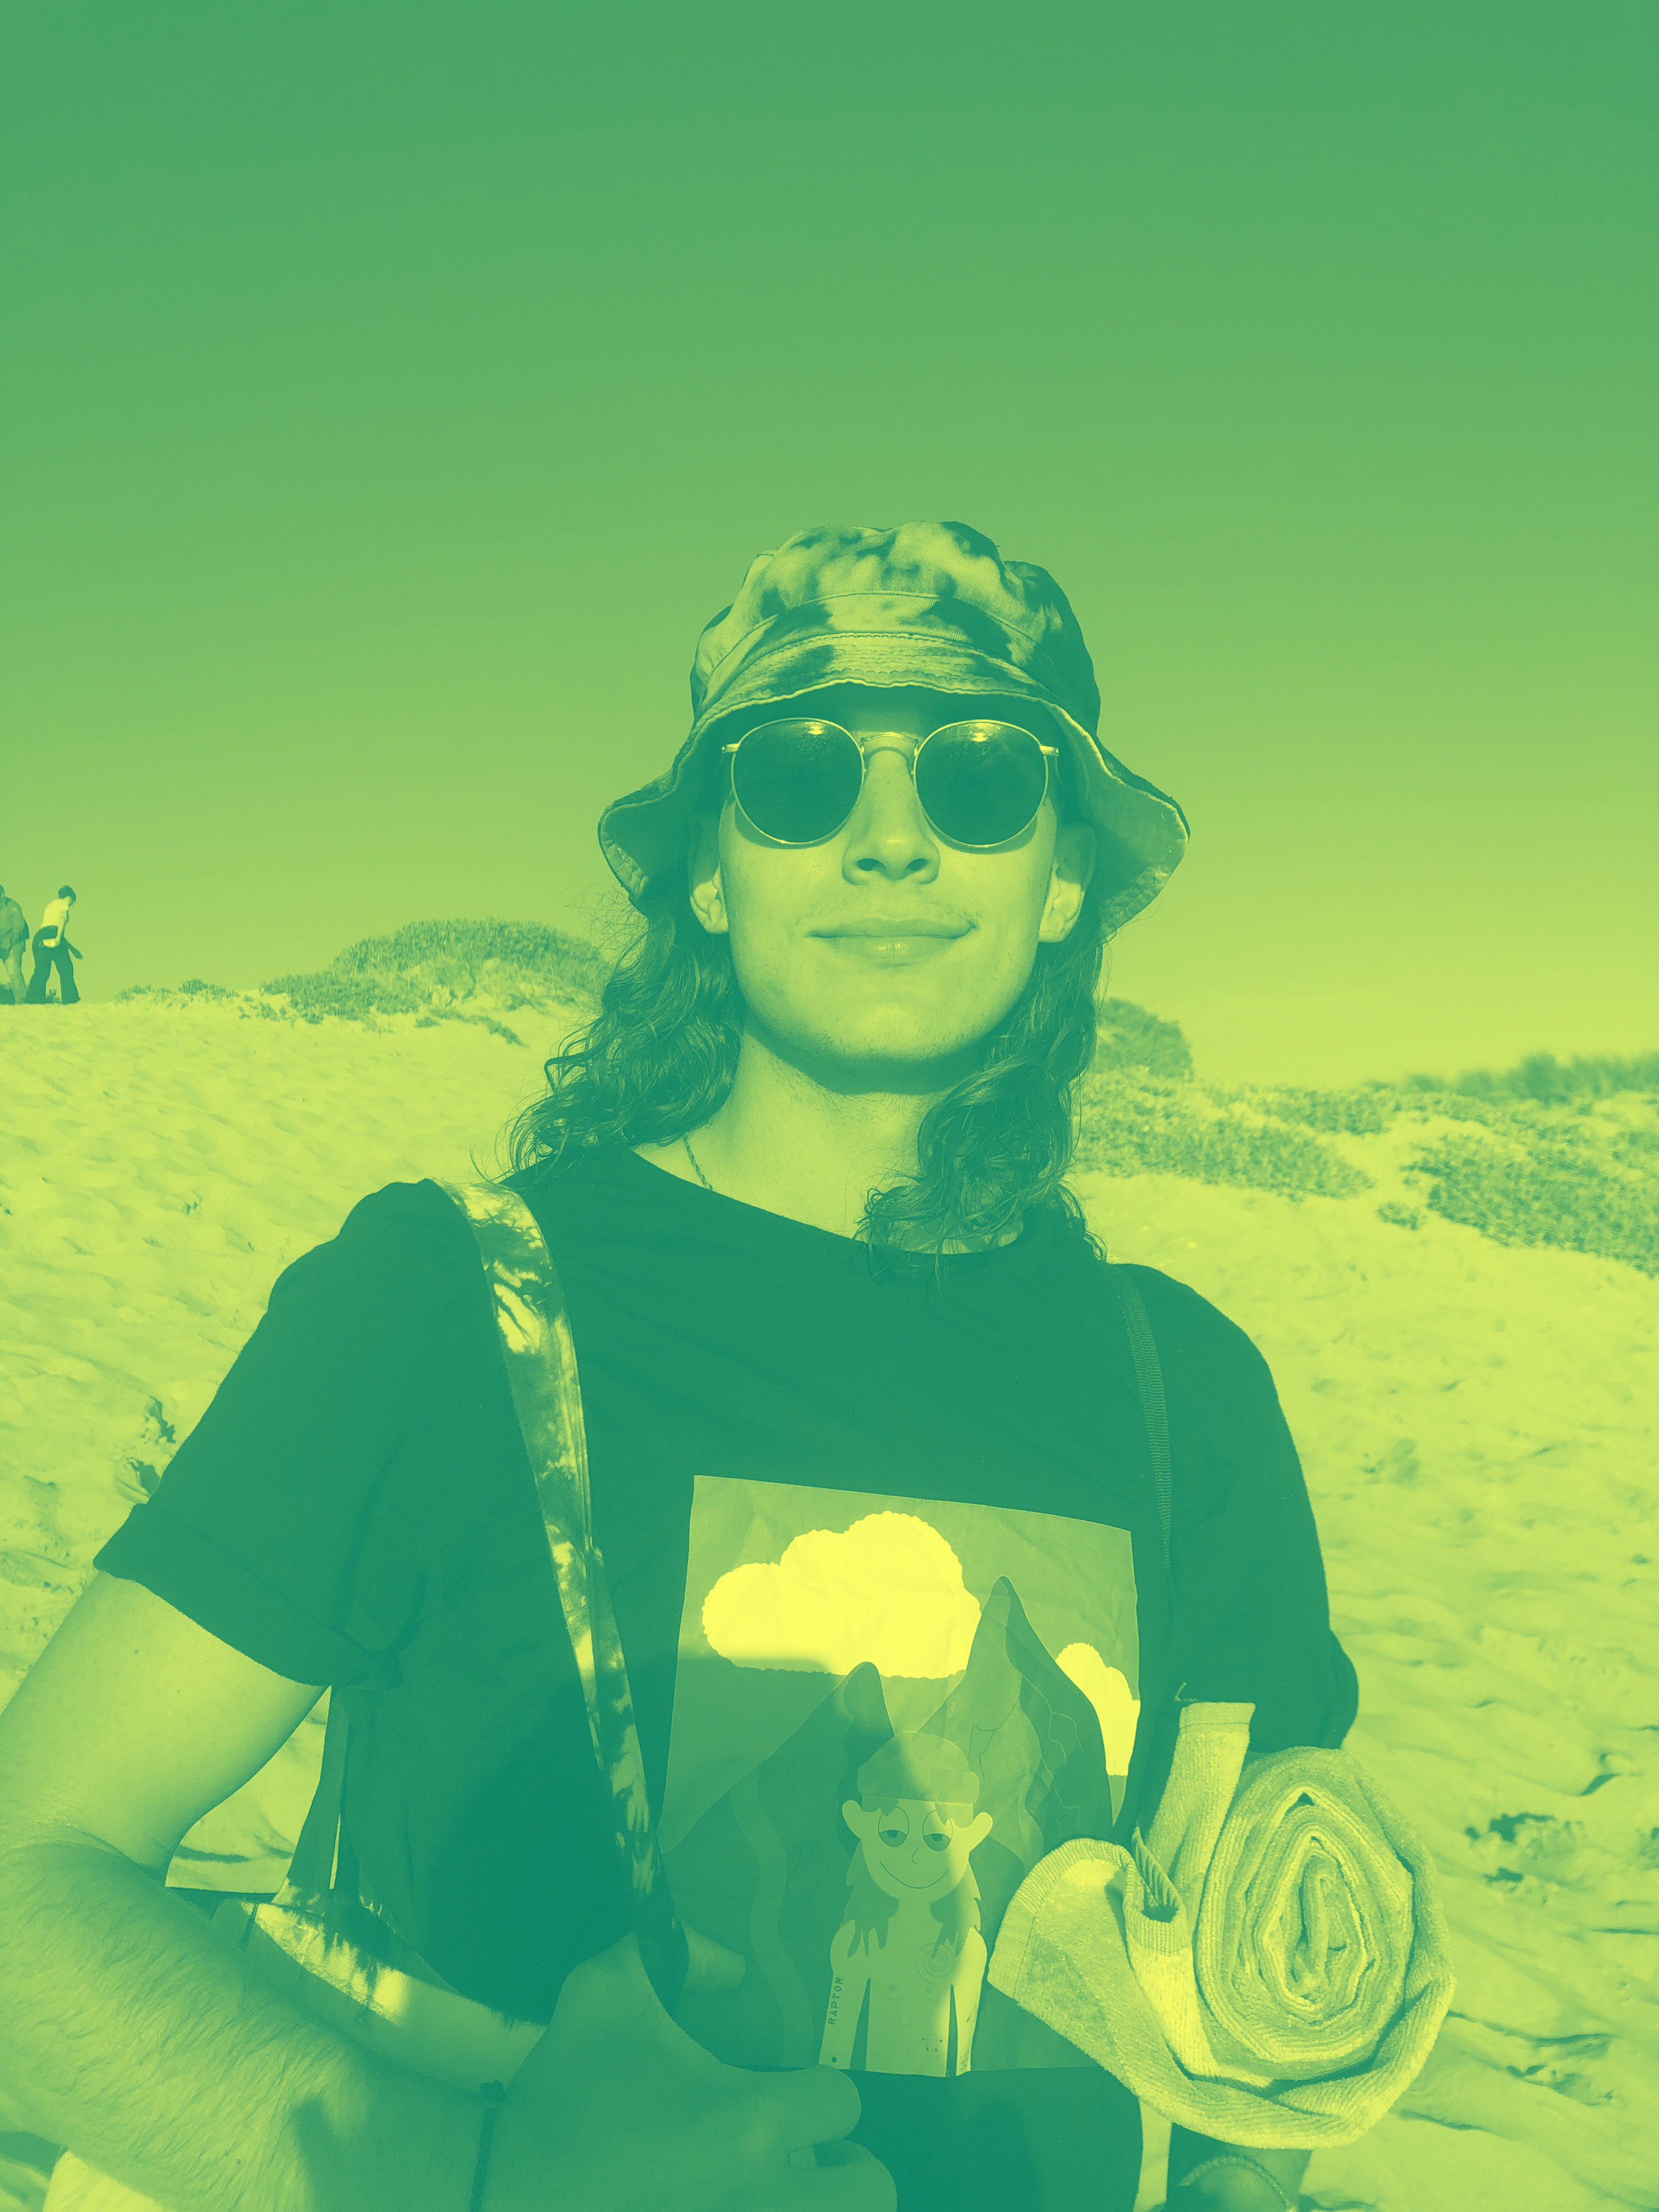
\includegraphics[width=.3\linewidth]{../Images/Output_Individual/Duo_Portrait.jpg}\label{Duo}}
	\subfloat[Thermal 1]{	\includegraphics[width=.3\linewidth]{../Images/Output_Individual/Thermal1_Portrait.jpg}\label{Thermal1}}
	\subfloat[Thermal 2]{	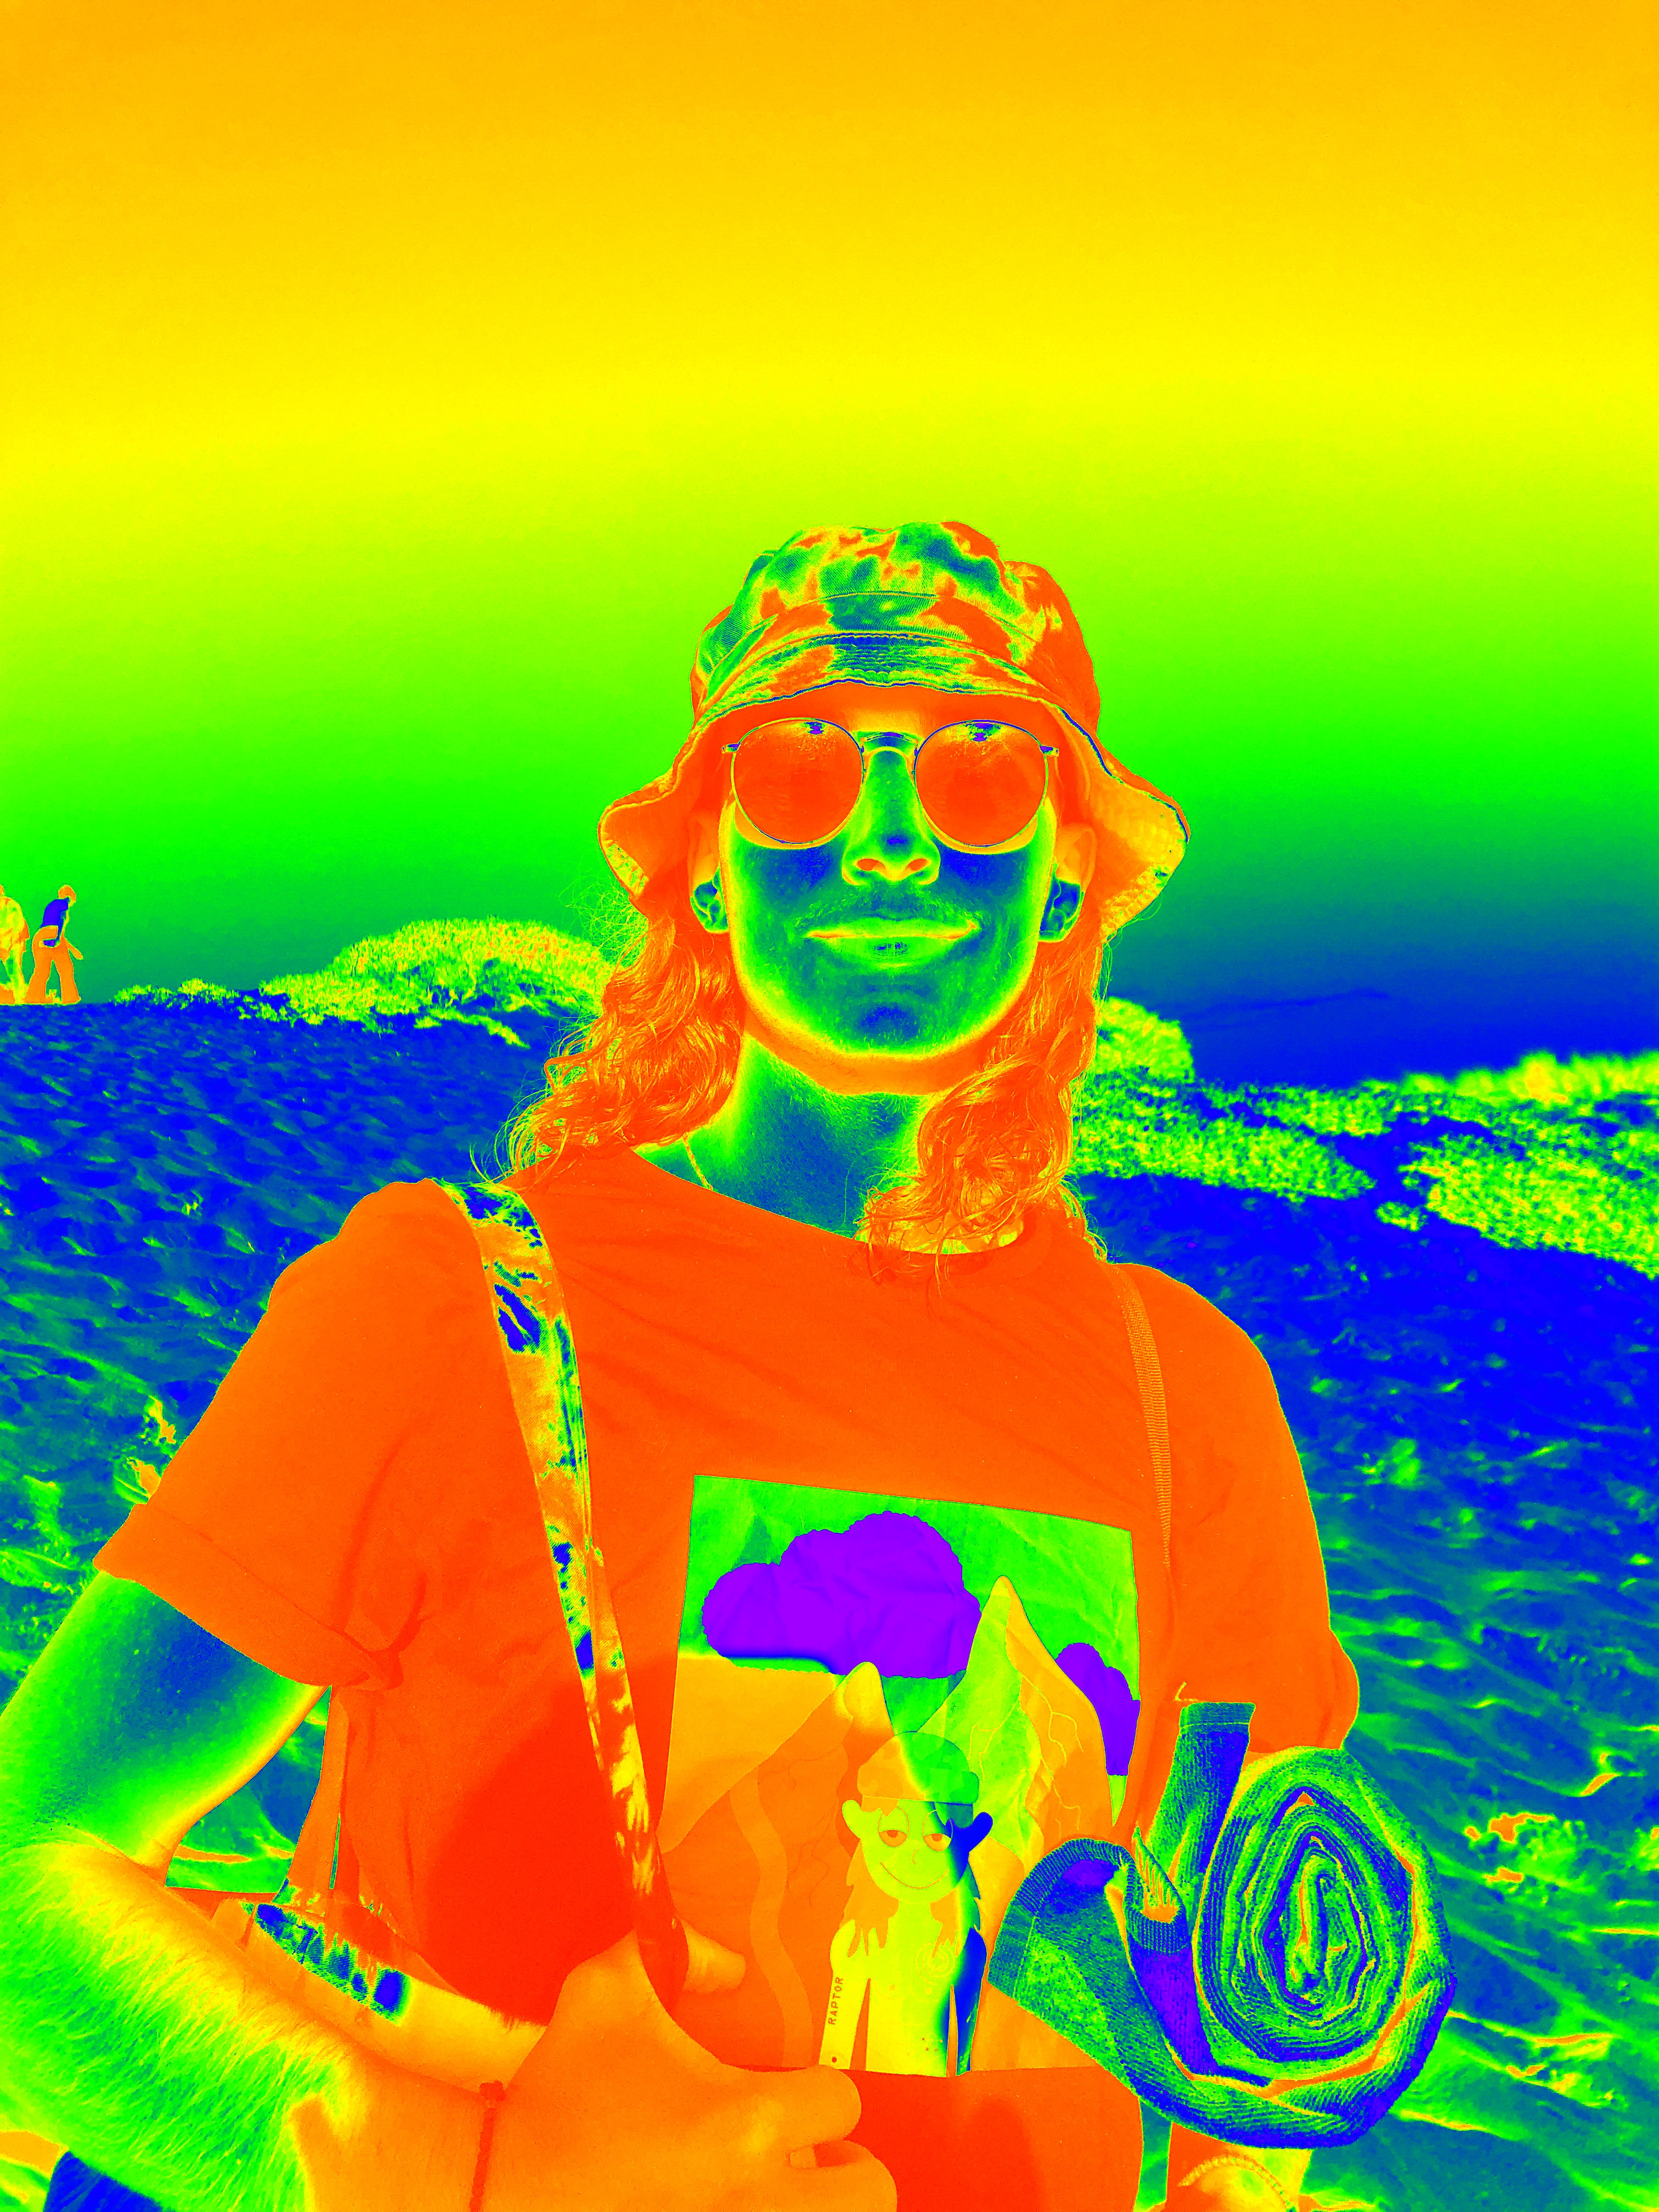
\includegraphics[width=.3\linewidth]{../Images/Output_Individual/Thermal2_Portrait.jpg}\label{Thermal2}}\\
	\subfloat[Thermal 3]{	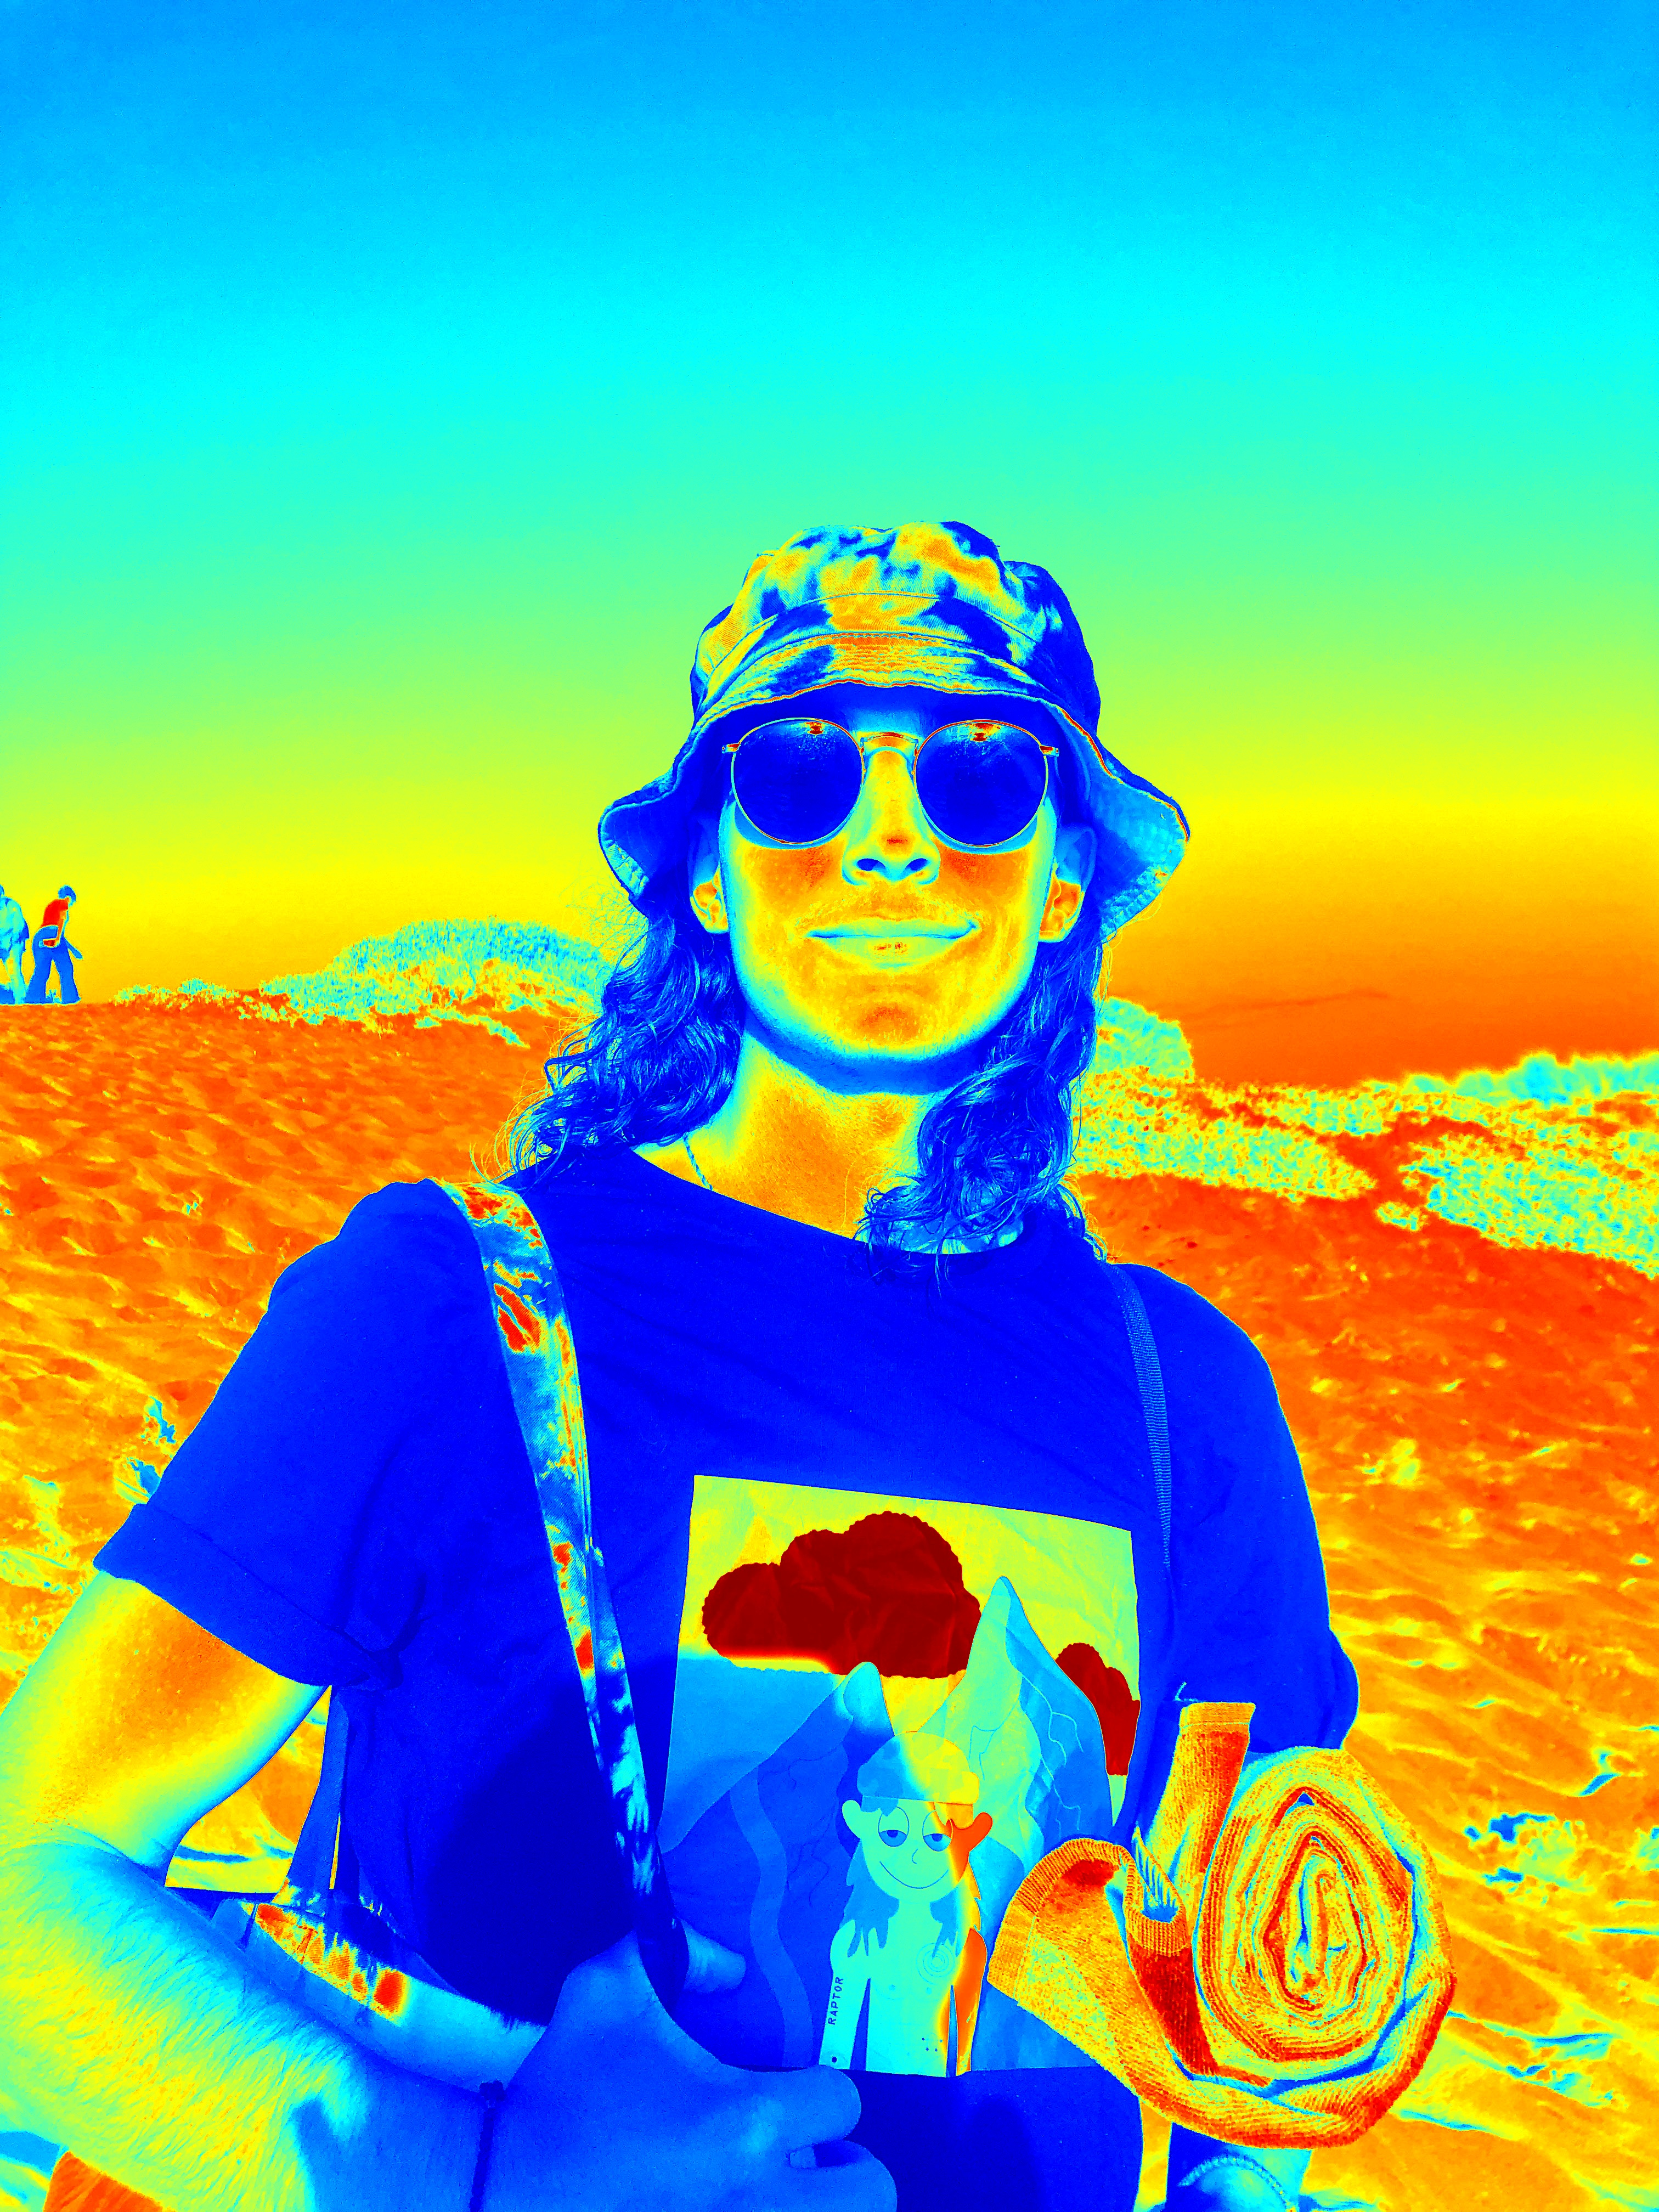
\includegraphics[width=.3\linewidth]{../Images/Output_Individual/Thermal3_Portrait.jpg}\label{Thermal3}}
	\subfloat[UV]{	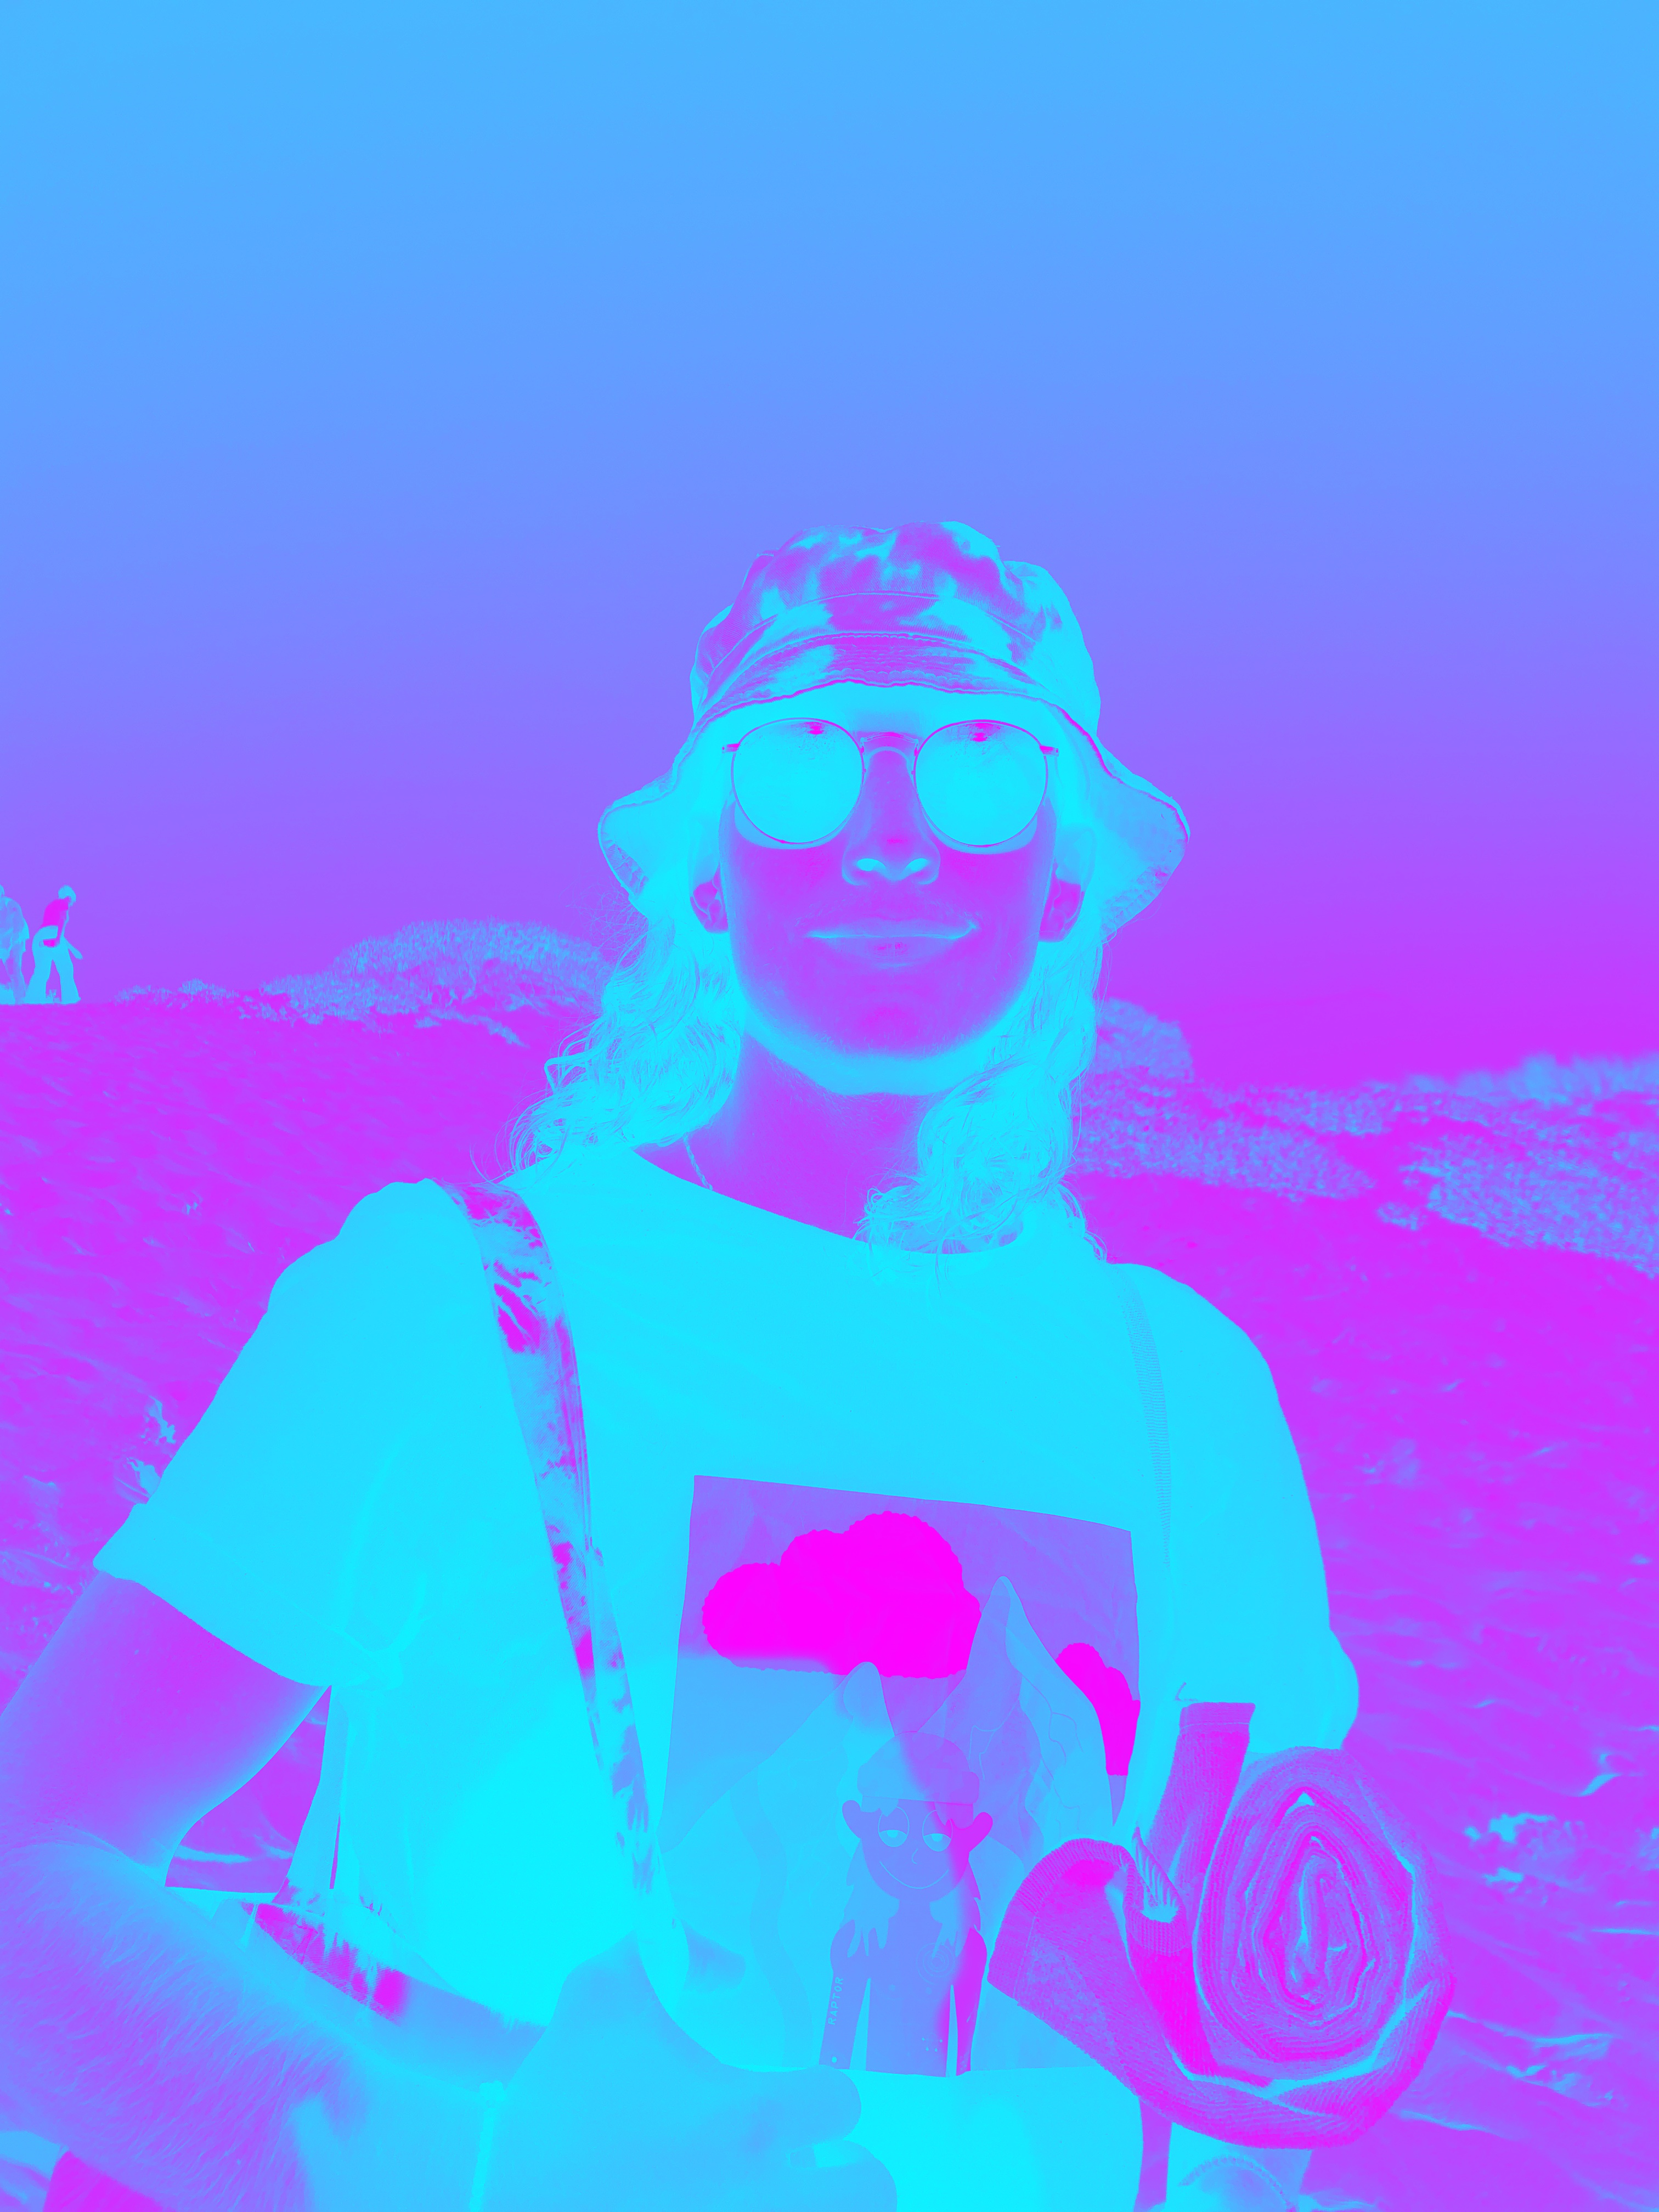
\includegraphics[width=.3\linewidth]{../Images/Output_Individual/UV_Portrait.jpg}\label{UV}}
	
	\caption{ColourMaps Results}
	\centering
	\label{Images_ColourMaps}
	\end{figure}

	
	\subsection{Extra Effect \#2 - WaterColor}
	Method used: cv2.stylization(img, sigma\_s=100, sigma\_r=0.9)\\
	As seen in Figure \ref{WaterColor}.
	\subsection{Extra Effect \#3 - Enhance}
	Method used: cv2.detailEnhance(img)\\
	As seen in Figure \ref{Enhance}.
	\subsection{Extra Effect \#4 - Glitch}
	This effect was implemented using a library called glitch\_this, by TotallyNotChase, found at \url{https://github.com/TotallyNotChase/glitch-this}. It is a command-line tool which reads in an image, and applies a glitch effect with a user-provided intensity, and optional scan lines too. I utilized the functionality in Jupyter that allows users to run terminal commands by using "!" before a line of code, and randomly generated the glitch intensity, and also whether or not the scan lines would be applied, in order to get varied results.
	As seen in Figure \ref{Glitch}.
	
	
	\begin{figure}[h]	
	\subfloat[WaterColor]{	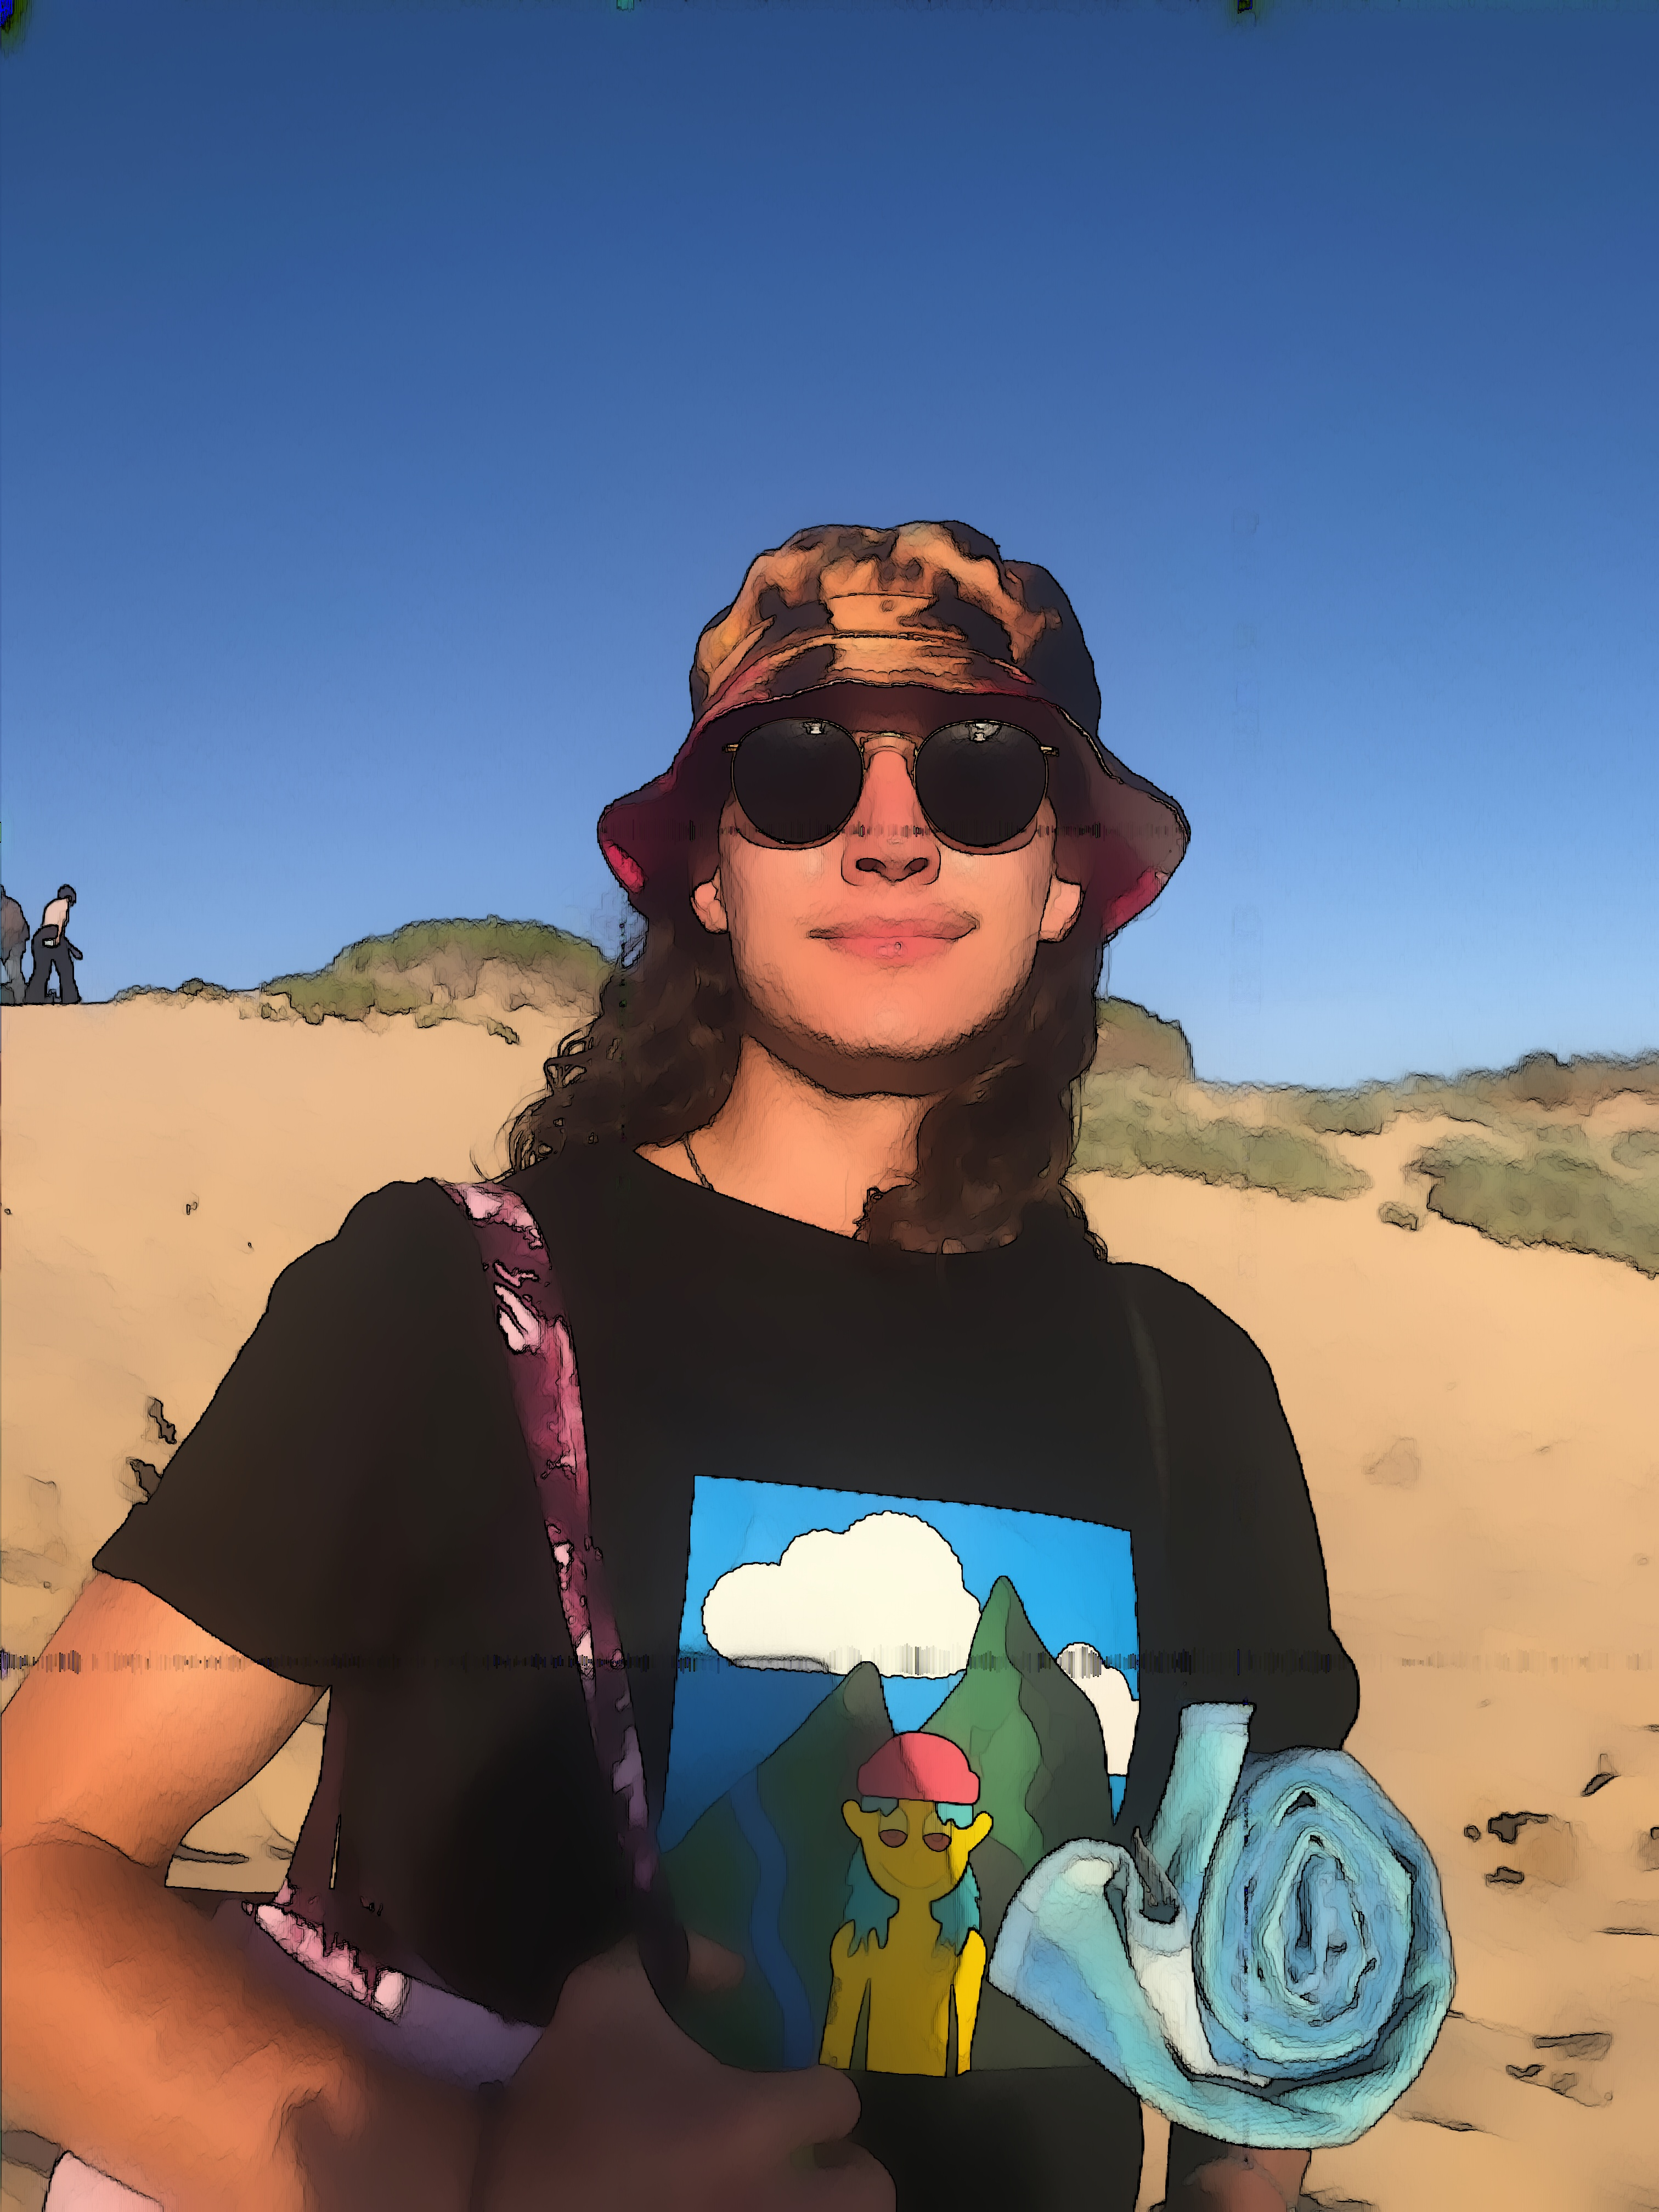
\includegraphics[width=.3\linewidth]{../Images/Output_Individual/WaterColour_Portrait.jpg}\label{WaterColor}}
	\subfloat[Enhance]{	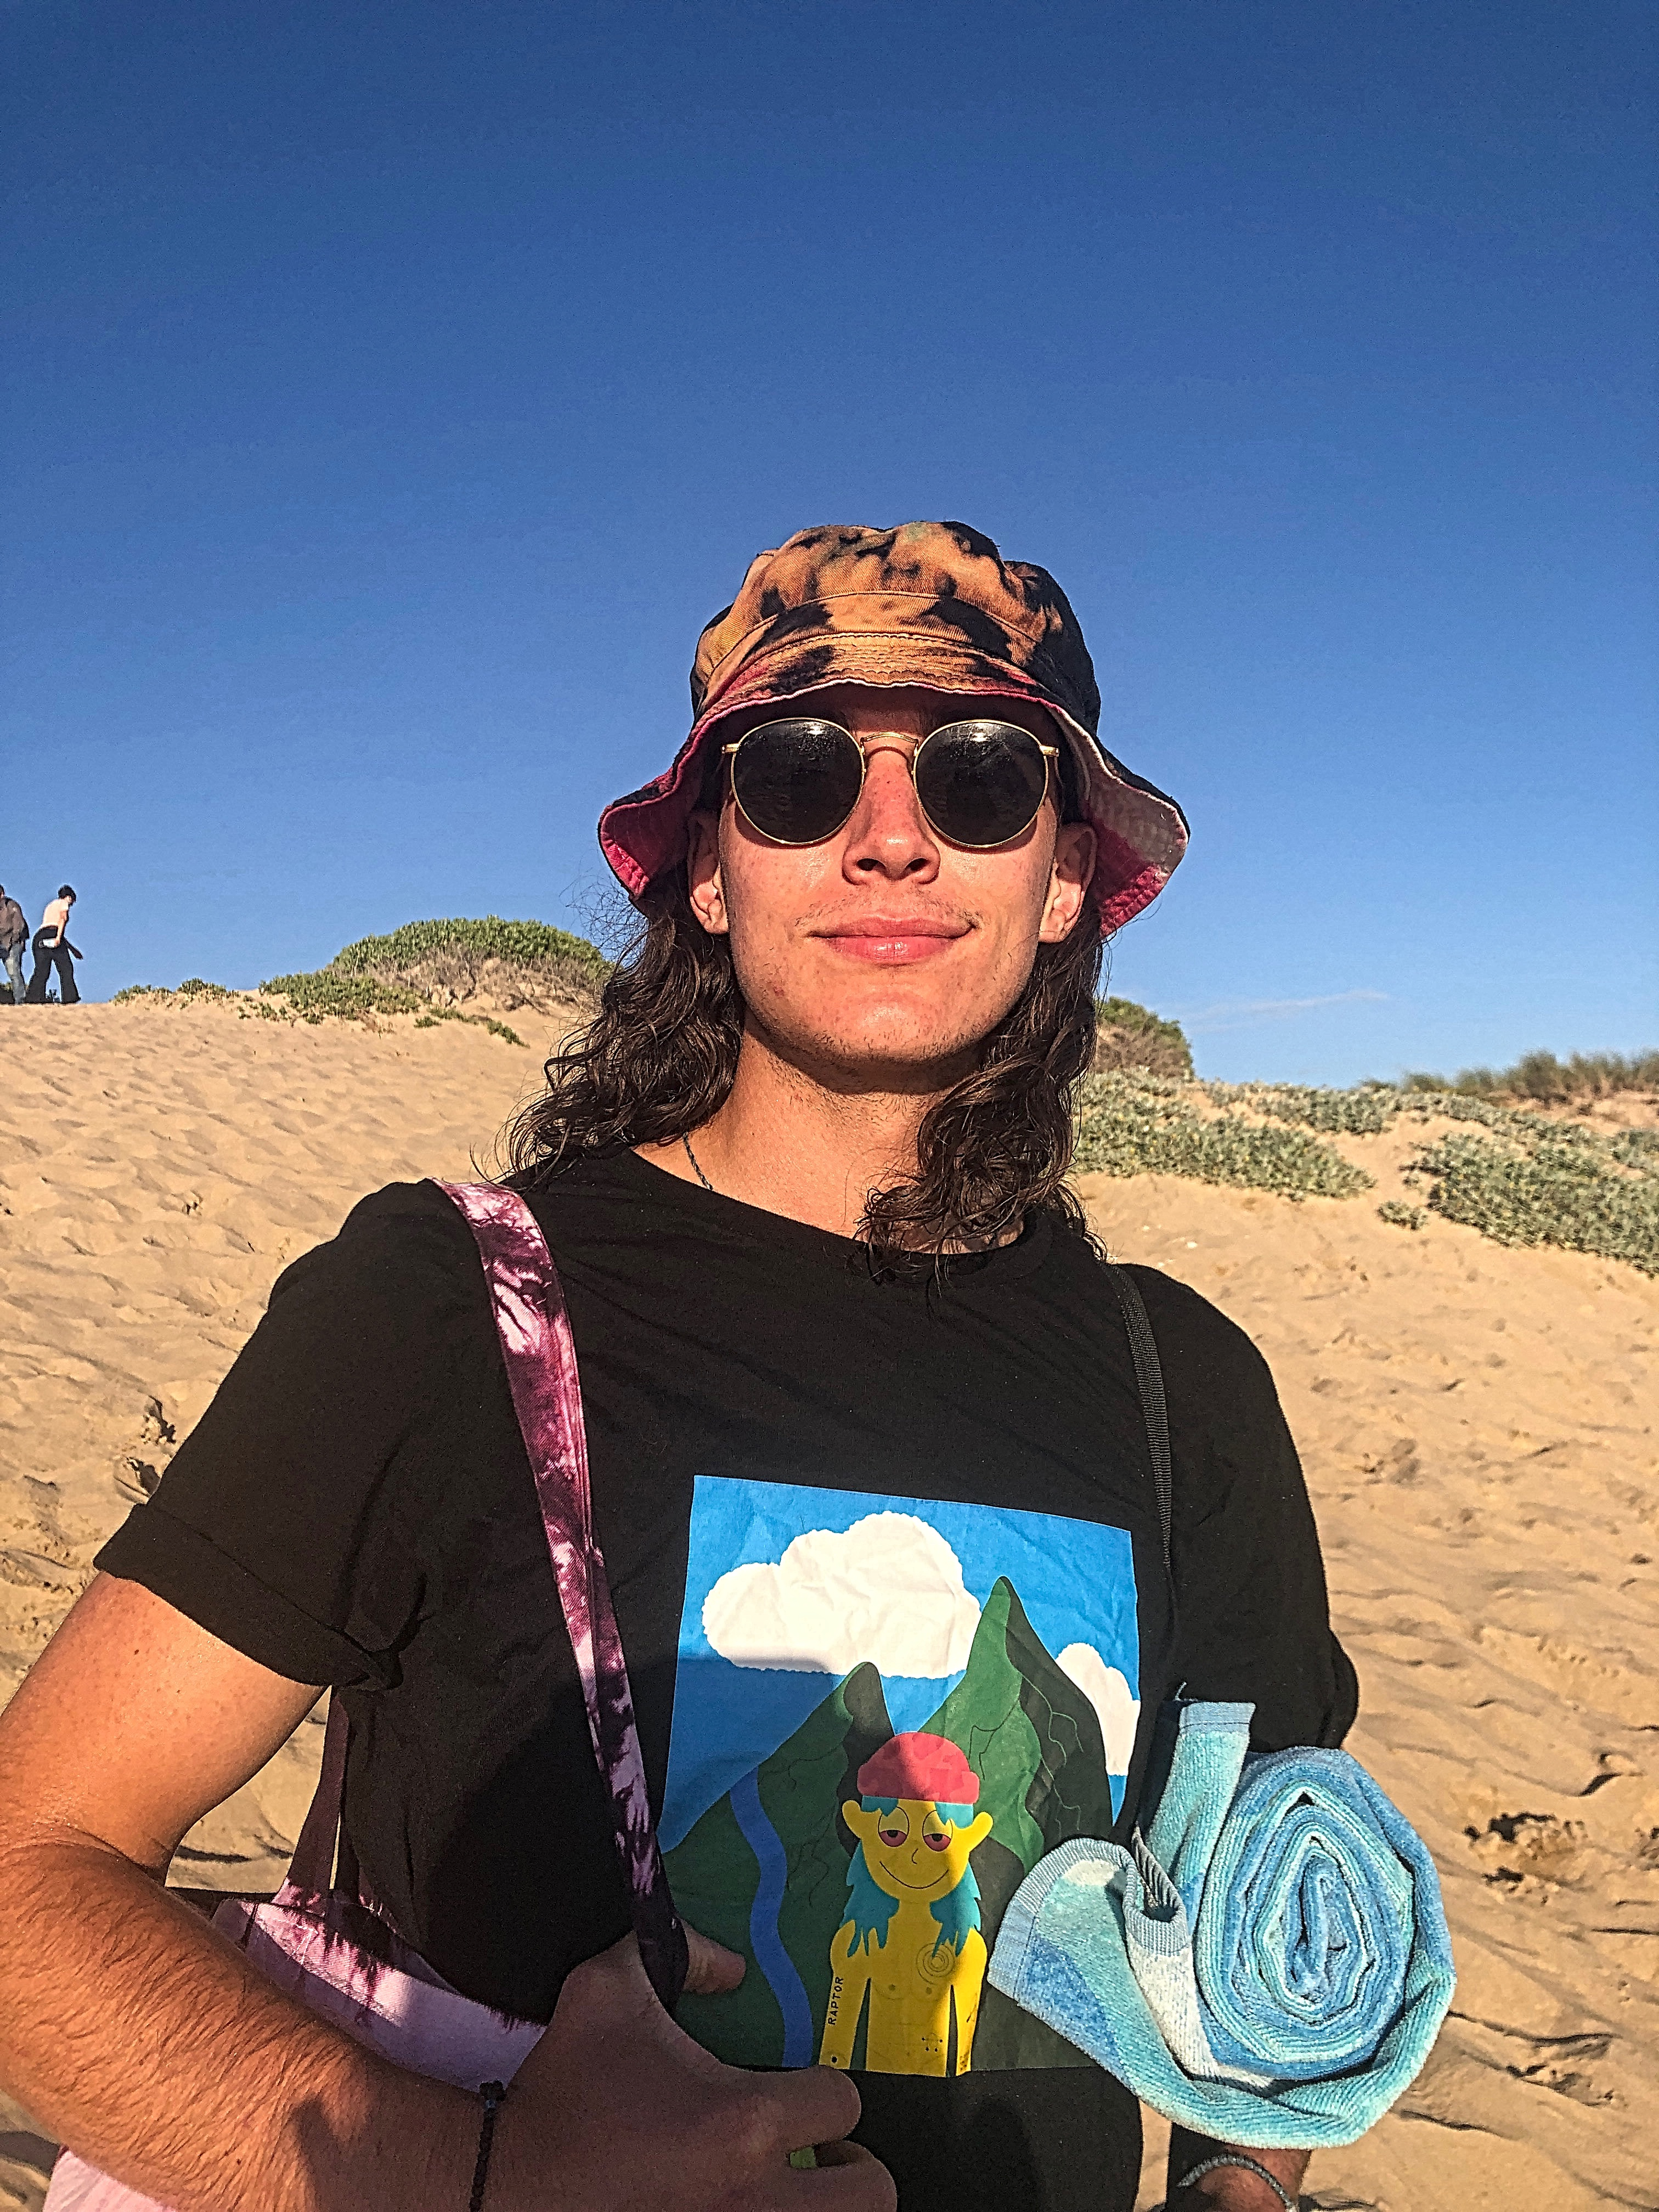
\includegraphics[width=.3\linewidth]{../Images/Output_Individual/Enhance_Portrait.jpg}\label{Enhance}}
	\subfloat[Glitch]{	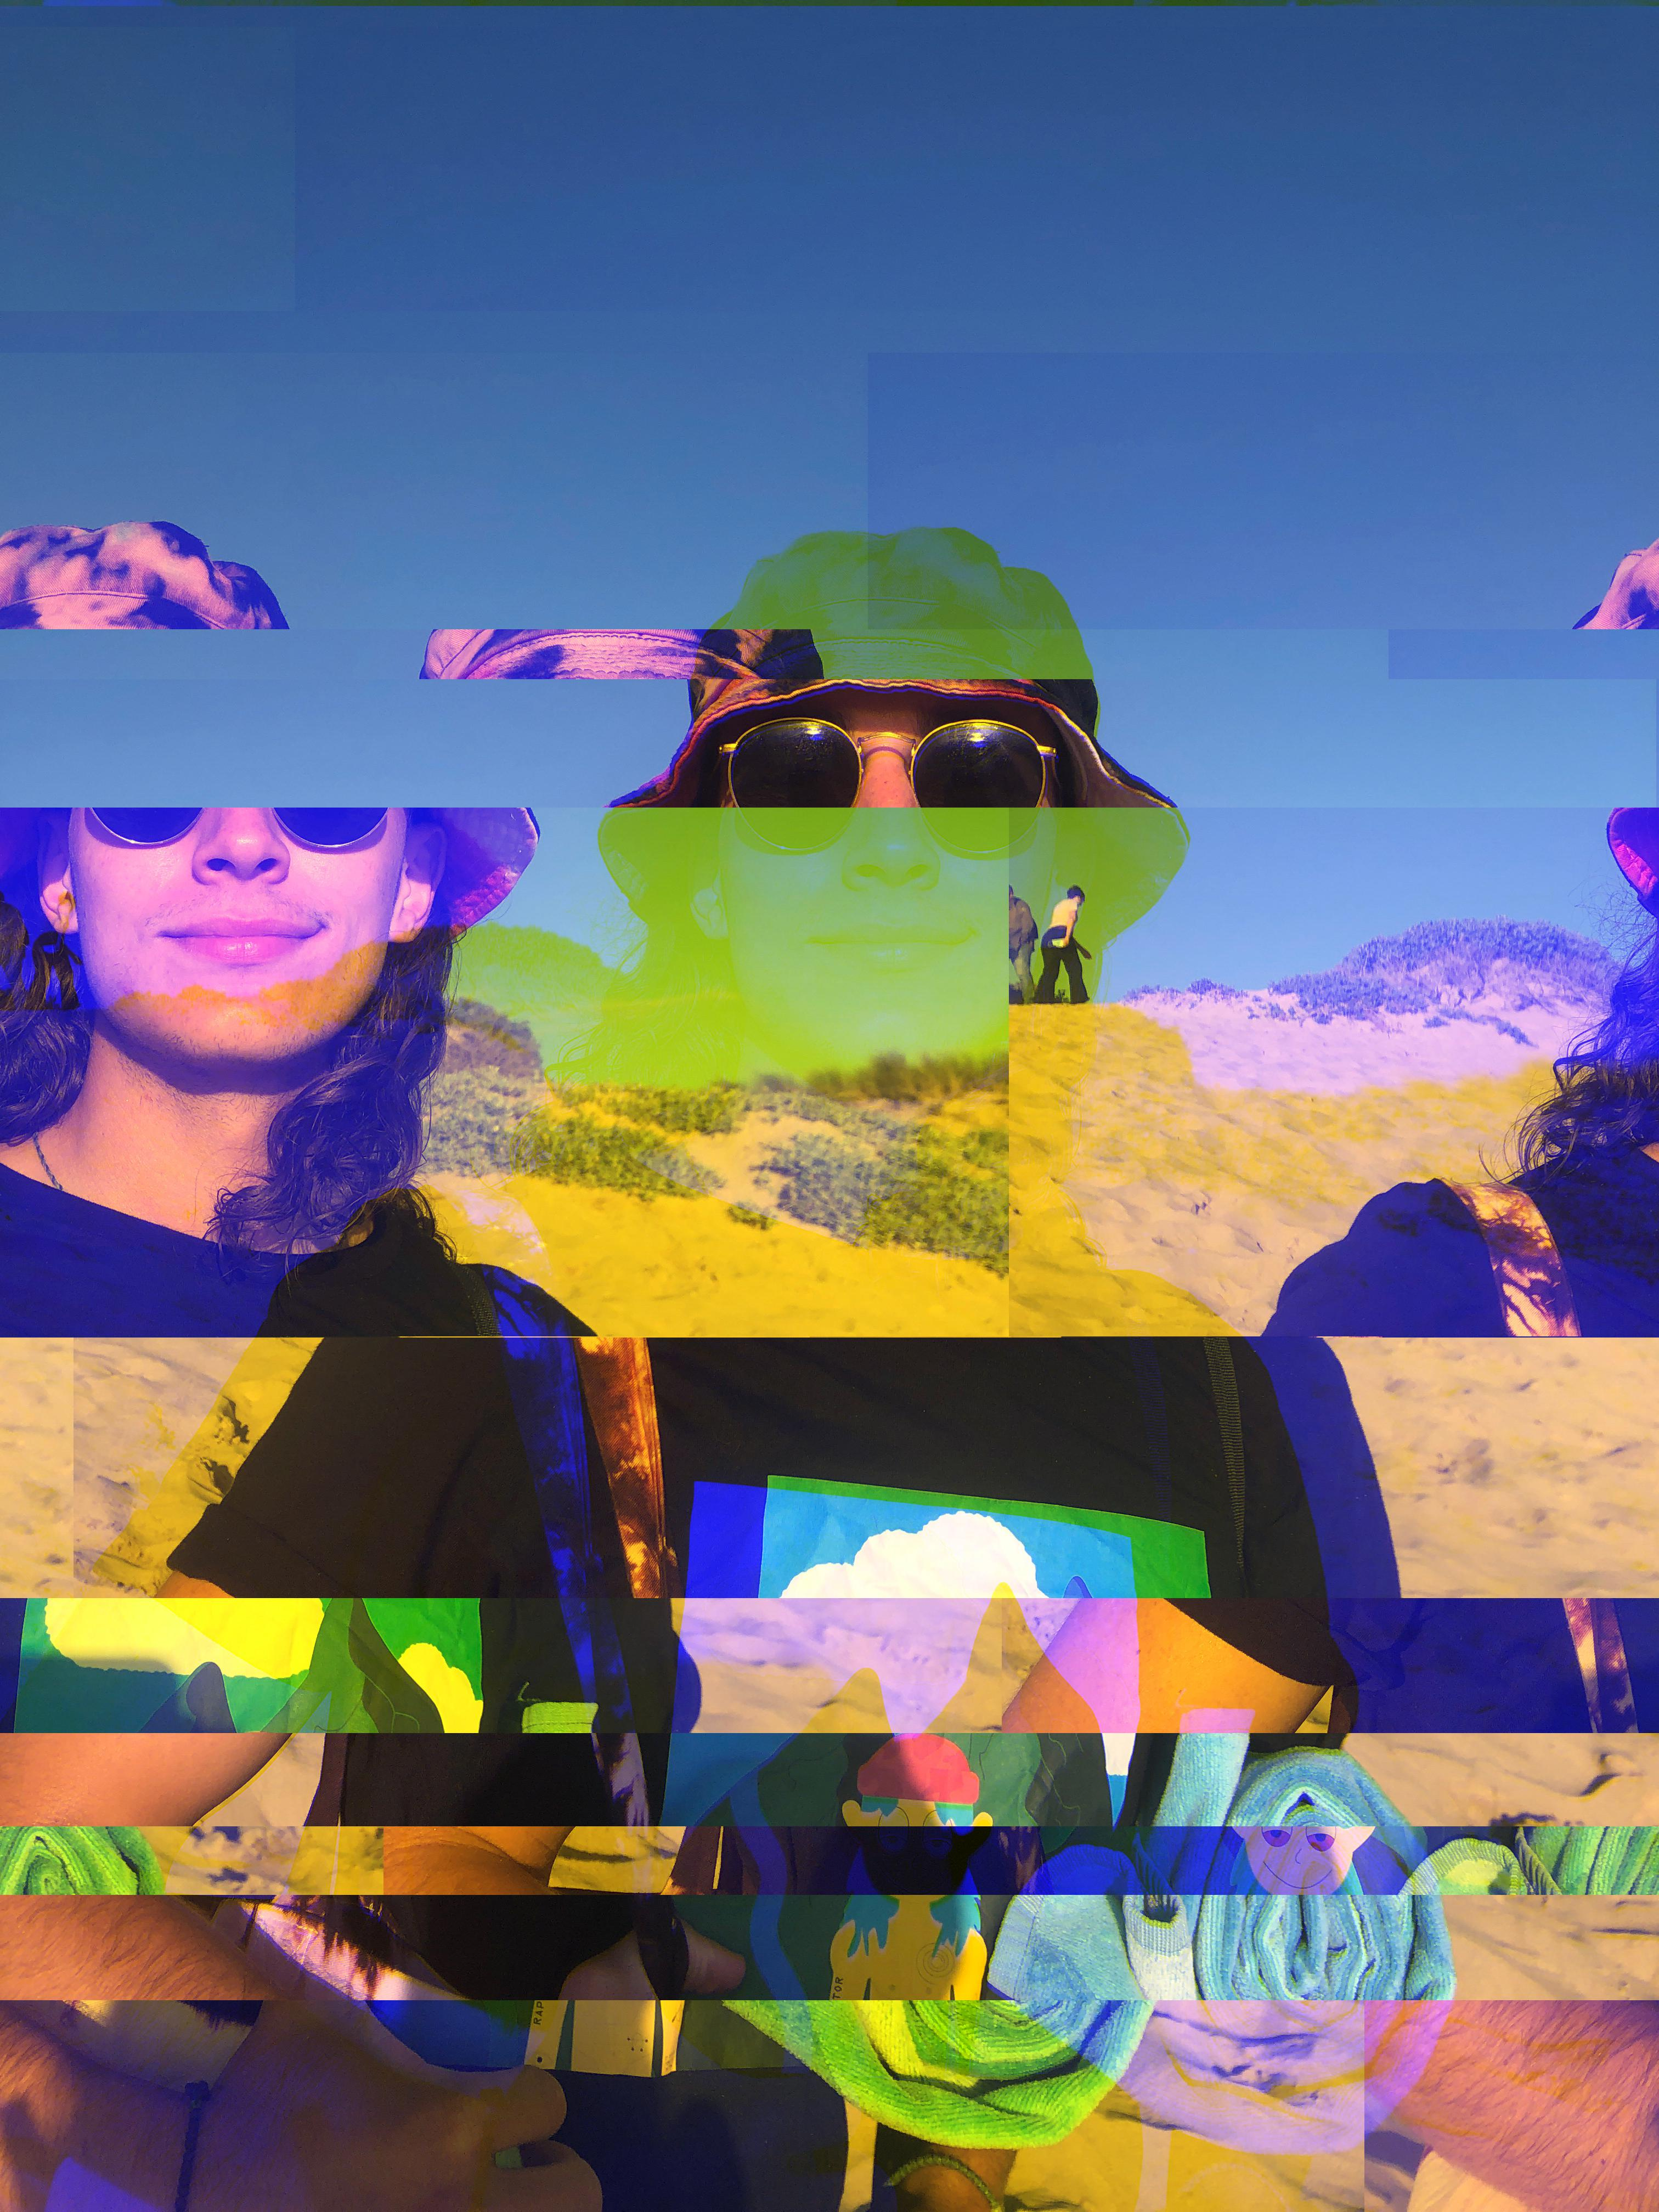
\includegraphics[width=.3\linewidth]{../Images/Output_Individual/Glitch_Portrait.jpg}\label{Glitch}}	
		
	\caption{Extra Effects}
	\centering
	\label{Images_ExtraEffects}
	\end{figure}
		
%	\nocite{*}
%	
%	\bibliography{references}\addcontentsline{toc}{chapter}{References}
%	
	\chapter{References}
	\begin{enumerate}
		\item \url{https://programmerbackpack.com/python-opencv-building-instagram-like-image-filters/}
		\item \url{https://python.joho.info/image-processing/opencv-emboss-filter-py/}
		\item \url{https://ulwazi.wits.ac.za/courses/12061/assignments/72155?module_item_id=217456}
		\item \url{https://github.com/mbeyeler/opencv-python-blueprints/blob/master/chapter1/filters.py}
		\item \url{https://analyticsindiamag.com/converting-an-image-to-a-cartoon/}
		\item \url{https://www.tutorialspoint.com/cartooning-an-image-using-opencv-in-python}
		\item \url{https://www.askaswiss.com/2016/01/how-to-create-cartoon-effect-opencv-python.html}
		\item \url{https://data-flair.training/blogs/cartoonify-image-opencv-python/}
		\item \url{https://subscription.packtpub.com/book/application_development/9781785282690/1/ch01lvl1sec12/cartoonizing-an-image}
		\item \url{https://towardsdatascience.com/turn-photos-into-cartoons-using-python-bb1a9f578a7e}
		\item \url{https://www.geeksforgeeks.org/cartooning-an-image-using-opencv-python/}
		\item \url{https://towardsdatascience.com/using-opencv-to-catoonize-an-image-1211473941b6}
		\item \url{http://datahacker.rs/002-opencv-projects-how-to-cartoonize-an-image-with-opencv-in-python/}
		\item \url{https://medium.com/boundlessinfo/a-mini-project-with-opencv-in-python-cartoonify-an-image-d82b9ff6df70}
		\item \url{https://jrtechs.net/data-science/creating-pixel-art-with-open-cv}
		\item \url{https://www.programmersought.com/article/2697972427/}
		\item \url{https://subscription.packtpub.com/book/application_development/9781785283932/2/ch02lvl1sec23/embossing}
		\item \url{https://stackoverflow.com/questions/55508615/how-to-pixelate-image-using-opencv-in-python}
		\item \url{https://www.freecodecamp.org/news/sketchify-turn-any-image-into-a-pencil-sketch-with-10-lines-of-code-cf67fa4f68ce/}	
		\item \url{https://medium.com/analytics-vidhya/create-your-own-sketch-with-opencv-638a463c6ec6}
		\item \url{https://analyticsindiamag.com/converting-image-into-a-pencil-sketch-in-python/}
		\item \url{https://bastelhalde.de/post/creating-fake-thermal-images-using-python}
	\end{enumerate}
	
	\appendix
    %APPENDIX A - MAIN
\chapter{Main Filters and Effects}
\label{MainEffects}

\begin{enumerate}
	\item Cartoonify
	\item Pencil Sketch
	\item Pixelate
	\item Emboss
\end{enumerate}


\begin{figure}[h]
	\caption{Cartoonify}
	\centering
	\includegraphics[width=\linewidth]{../Images/Output_All/ALL_Cartoonify.jpg}
	\label{ALLCartoonify}
\end{figure}


\begin{figure}[h]
	\caption{Pencil Sketch}
	\centering
	\includegraphics[width=\linewidth]{../Images/Output_All/ALL_Pencil_Sketch.jpg}
	\label{ALLPencilSKetch}
\end{figure}


\begin{figure}[h]
	\caption{Pixelate}
	\centering
	\includegraphics[width=\linewidth]{../Images/Output_All/ALL_Pixelate.jpg}
	\label{ALLPixelate}
\end{figure}

\begin{figure}[h]
	\caption{Emboss}
	\centering
	\includegraphics[width=\linewidth]{../Images/Output_All/ALL_Emboss.jpg}
	\label{ALLEmboss}
\end{figure}





%APPENDIX B - EXTRA
\chapter{Extra Filters and Effects}
\label{ExtraEffects}

\begin{itemize}
	\item ColorMaps
	\begin{itemize}
		\item Duo Chromatic
		\item Thermal 1
		\item Thermal 2
		\item Thermal 3
		\item UV
	\end{itemize}
	\item WaterColor
	\item Enhance
	\item Glitch
\end{itemize}

\begin{figure}[h]
	\caption{Duo Chromatic}
	\centering
	\includegraphics[width=\linewidth]{../Images/Output_All/ALL_Duo.jpg}
	\label{ALLDuo}
\end{figure}

\begin{figure}[h]
	\caption{Thermal1}
	\centering
	\includegraphics[width=\linewidth]{../Images/Output_All/ALL_Thermal1.jpg}
	\label{ALLThermal1}
\end{figure}

\begin{figure}[h]
	\caption{Thermal2}
	\centering
	\includegraphics[width=\linewidth]{../Images/Output_All/ALL_Thermal2.jpg}
	\label{ALLThermal2}
\end{figure}

\begin{figure}[h]
	\caption{Thermal3}
	\centering
	\includegraphics[width=\linewidth]{../Images/Output_All/ALL_Thermal3.jpg}
	\label{ALLThermal3}
\end{figure}

\begin{figure}[h]
	\caption{UV}
	\centering
	\includegraphics[width=\linewidth]{../Images/Output_All/ALL_UV.jpg}
	\label{ALLUV}
\end{figure}

\begin{figure}[h]
	\caption{WaterColor}
	\centering
	\includegraphics[width=\linewidth]{../Images/Output_All/ALL_WaterColour.jpg}
	\label{ALLWaterColor}
\end{figure}

\begin{figure}[h]
	\caption{Enhance}
	\centering
	\includegraphics[width=\linewidth]{../Images/Output_All/ALL_Enhance.jpg}
	\label{ALLEnhance}
\end{figure}

\begin{figure}[h]
	\caption{Glitch}
	\centering
	\includegraphics[width=\linewidth]{../Images/Output_All/ALL_Glitch.jpg}
	\label{ALLGlitch}
\end{figure}
	

\end{document}
